Dai macroblocchi delle entità fondamentali possiamo costruire un primo schema scheletro che descriva le relazioni essenziali e da questo poi sviluppare un modello più complesso.\newline



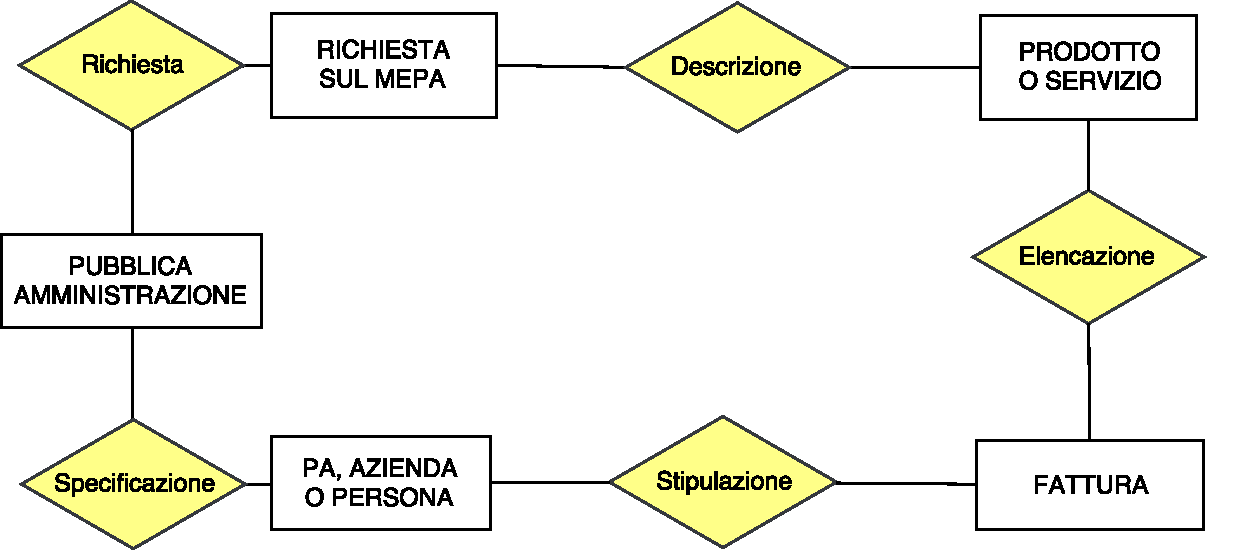
\includegraphics[width=0.7\linewidth]{./immagini/schema_scheletro.pdf}

\newline
Si può vedere come le relazioni inserite nello schema scheletro formino un sistema chiuso, il che mette in risalto l'interconnessione tra le diverse entità che deriva ed è rappresentata dallo schema dei processi interni che qui specifica in maniera più schematica le relazioni che vi sono tra le diverse componenti del processo.